\documentclass[11pt,a4paper]{article}
\usepackage[utf8]{inputenc}
\usepackage[spanish]{babel}	%Idioma
\usepackage{amsmath}
\usepackage{amsfonts}
\usepackage{amssymb}
\usepackage{graphicx} %Añadir imágenes
\usepackage{geometry}	%Ajustar márgenes
\usepackage[export]{adjustbox}[2011/08/13]
\usepackage{float}
\restylefloat{table}
\usepackage{hyperref}
\usepackage{titling}
%\usepackage{minted}
\usepackage[font=small,labelfont=bf]{caption} 

%Opciones de encabezado y pie de página:
\usepackage{fancyhdr}
\pagestyle{fancy}
\lhead{}
%\rhead{}
\lfoot{Desarrollo Basado en Agentes}
\cfoot{}
\rfoot{\thepage}
\renewcommand{\headrulewidth}{0.4pt}
\renewcommand{\footrulewidth}{0.4pt}

%Opciones de fuente:
\usepackage[utf8]{inputenc}
\usepackage[default]{sourcesanspro}
\usepackage{sourcecodepro}
\usepackage[T1]{fontenc}


\setlength{\parindent}{0pt}
\setlength{\headheight}{15pt}
\setlength{\voffset}{10mm}

% Custom colors
\usepackage{color}
\definecolor{deepblue}{rgb}{0,0,0.5}
\definecolor{deepred}{rgb}{0.6,0,0}
\definecolor{deepgreen}{rgb}{0,0.5,0}

\usepackage{listings}

% Evitar guiones al final de línea.
%\tolerance=1
%\emergencystretch=\maxdimen
%\hyphenpenalty=10000
%\hbadness=10000

\pretitle{%
  \centering
  \LARGE
  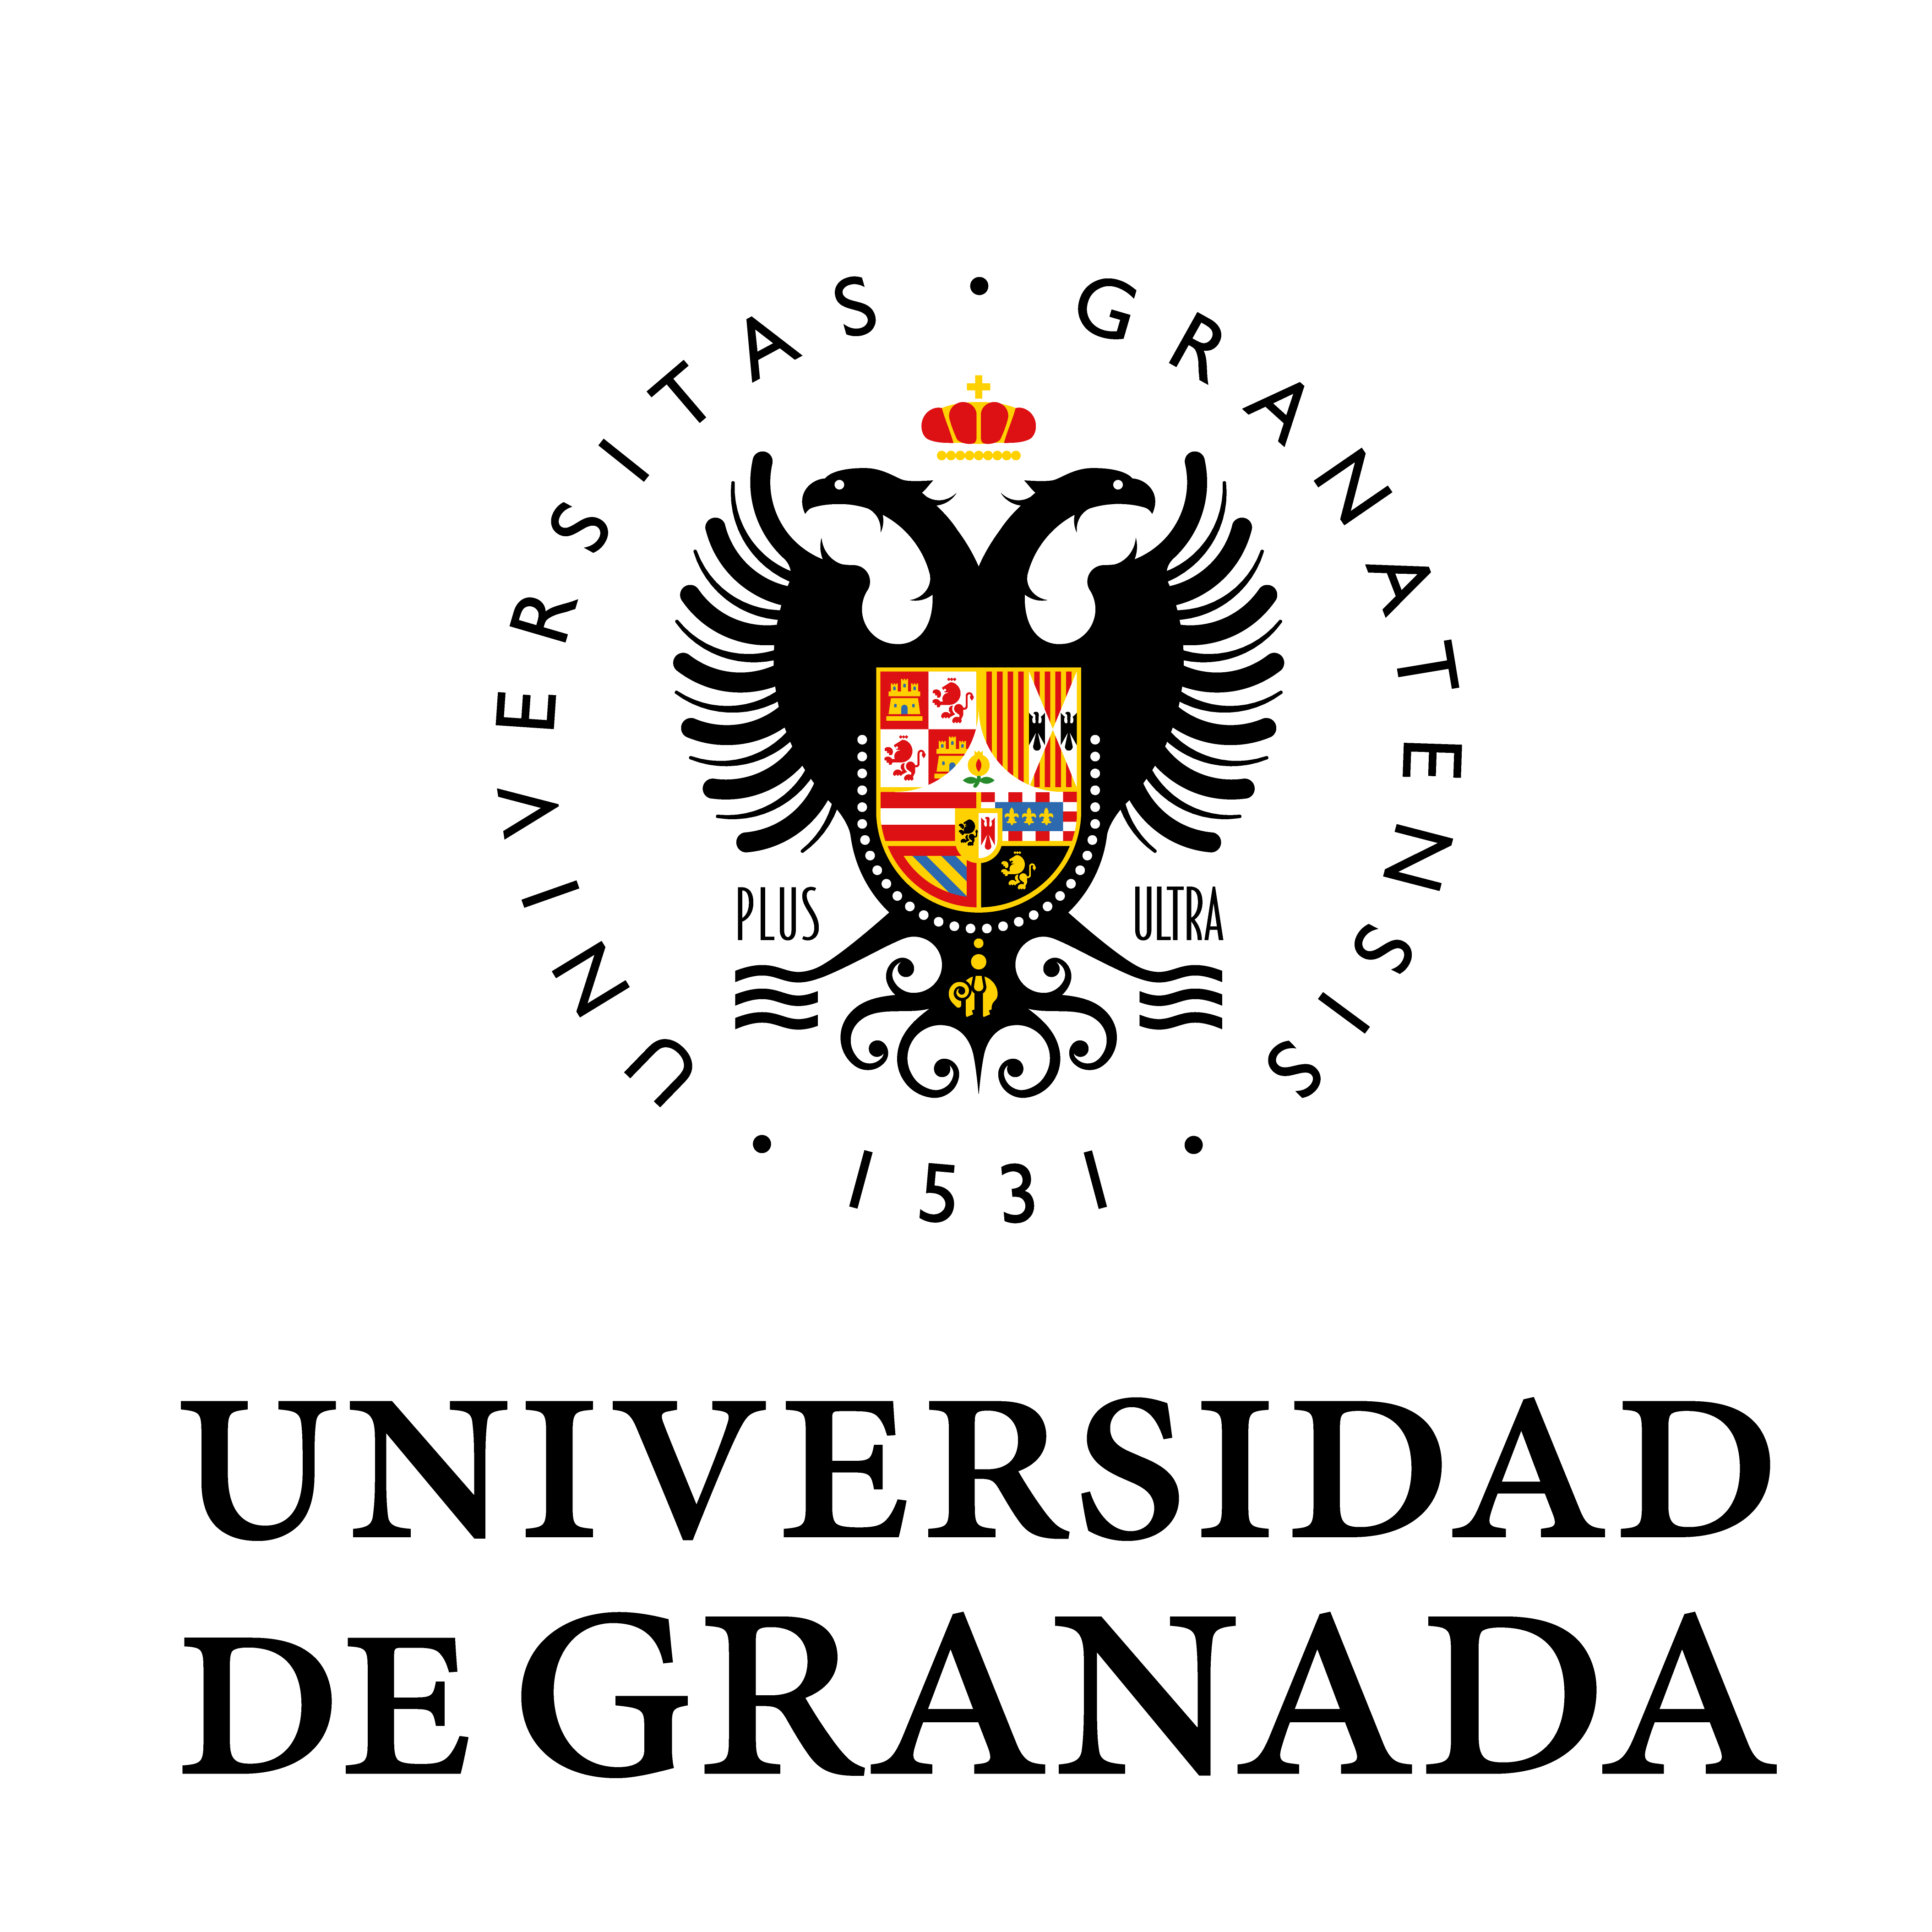
\includegraphics[scale=0.5]{img/logo.png}\\[\bigskipamount]
}
\posttitle{\begin{center} \end{center}}

\author{Guillermo Bueno Vargas \\ Bruno García Trípoli \\ Alberto Gurrea Callejas \\ Juan Ocaña Valenzuela}
\title{\textbf{Desarrollo Basado en Agentes} \\ 
 Práctica 2: misión DRAGONFLY}

%%%%%%%%%%%%%%%%%%%%%%%%%%%%%%%%%%%%%%%%%%%%%%%%%%%%%%%%%%%%%%%%%%%%%%%%%%%%%%%
%% EL DOCUMENTO EMPIEZA AQUÍ
%%%%%%%%%%%%%%%%%%%%%%%%%%%%%%%%%%%%%%%%%%%%%%%%%%%%%%%%%%%%%%%%%%%%%%%%%%%%%%%

\begin{document}

\thispagestyle{empty}

\maketitle

\begin{center}

Versión: 1.0
\end{center}

\newpage

Esta obra está sujeta a la licencia Reconocimiento-NoComercial-CompartirIgual 4.0 Internacional de Creative Commons. Para ver una copia de esta licencia, visite 

\url{http://creativecommons.org/licenses/by-nc-sa/4.0/}.

\bigskip


\includegraphics[scale=2]{img/by-nc-sa.png}\\[\bigskipamount]

\newpage

\tableofcontents

\newpage

\section{Descripción del problema}

El problema a abordar consiste en diseñar e implementar el comportamiento de la sonda \textit{Dragonfly}, que ha de moverse en un entorno hostil hacia una zona establecida 
haciendo uso de diferentes sensores.

El agente ha de cumplir los siguientes requisitos:

\begin{itemize}
	 \item Desplazarse de forma autónoma guiado por los sensores activos hacia el objetivo.
	 \item Evitar colisiones con el relieve del mundo.
	 \item Evitar que se agote la batería, recargando cuando sea necesario.
	 \item Una vez llegado al objetivo, posarse sobre él.
\end{itemize}

Para realizar todo esto, el agente ha de comunicarse con un controlador específico, que le informará de los resultados de sus acciones y la información actualizada
de sus sensores mediante un mensaje codificado en JSON. El agente ha de decodificar estos datos, actualizando su base de conocimiento y haciendo uso de ella para 
volver a actuar.

\section{Diseño del agente}

A continuación se adjuntan los diferentes diagramas utilizados en la implementación del funcionamiento del agente:
\begin{itemize}
	\item Diagrama de clases: https://drive.google.com/open?id=1AVGlVi7iFwF_wf06LgfKT3ENoQBaMscI
	\item Diagrama de comunicación: https://drive.google.com/open?id=1Np2DMOF74VwDmPBNyue3_3VKu_a10eLy
	\item Diagrama de actividad: https://drive.google.com/open?id=1IwIZwNYwJSlLvSVjxOjM7ngV2bpRHg42
\end{itemize}

\section{Lógica del agente}

Se ha optado por una solución \textit{greedy} utilizando los sensores \textbf{GPS}, \textbf{RADAR}, \textbf{ELEVATION}, \textbf{GONIO} y \textbf{MAGNETIC}.

El proceso de actuación es el siguiente:

\begin{enumerate}
	\item Registrar que ha pasado por una casilla, sumando uno en la correspondiente posición de la matriz de huellas.
	\item Comprobar si alguna de las posiciones de su alrededor presenta peligro de dejar al agente sin batería al avanzar por ese camino. Si es así, se activa el modo \textit{onRefuel}, en el que:
	
	\begin{itemize}
		\item Si no está posado en el suelo, desciende.
		\item Si está posado en el suelo, recarga y sale del modo \textit{onRefuel}.
	\end{itemize}
	
	\item Si no está en modo \textit{onRefuel}  ni detecta la meta debajo, se mueve de la siguiente forma:
	\begin{enumerate}
		\item Divide el espacio horizontal en octantes cuyo origen es la posición GPS del agente, y detecta en cuál se halla el objetivo con el ángulo de \textbf{GONIO}, asignando mayor peso a los movimientos cuanto mayor ángulo formen con él.
		\item Se comprueba si es posible moverse hacia una casilla determinada relativa a la posición del drone de entre las detectadas en los sensores, comprobando también su altura, y penalizando levemente la acción si conlleva desplazarse a una casilla cuya altitud es mayor a la actual. Esta valoración se suma a la anterior.
		\item Se selecciona el movimiento a la casilla con menor valor, y el movimiento correspondiente. Si la casilla se encuentra a mayor altitud que el agente, se realiza un movimiento hacia arriba.
	\end{enumerate}
\end{enumerate}

\section{Resultados observados}


\end{document}
